% \documentclass{article}
\documentclass[acmlarge, review=false, screen=true]{acmart}

\usepackage[utf8]{inputenc} 
\usepackage{natbib}
% \usepackage{a4wide}
\usepackage{url}

\citestyle{acmnumeric}
\bibliographystyle{ACM-Reference-Format}

\AtBeginDocument{%
  \providecommand\BibTeX{{%
    \normalfont B\kern-0.5em{\scshape i\kern-0.25em b}\kern-0.8em\TeX}}}

%% Rights management information.  This information is sent to you
%% when you complete the rights form.  These commands have SAMPLE
%% values in them; it is your responsibility as an author to replace
%% the commands and values with those provided to you when you
%% complete the rights form.
% \setcopyright{acmcopyright}
\setcopyright{none}
% \copyrightyear{2018}
% \acmYear{2018}
% \acmDOI{10.1145/1122445.1122456}
\acmDOI{} % This was required so I left it empty    /Casper


%%
%% These commands are for a JOURNAL article.
% \acmJournal{POMACS}
% \acmVolume{37}
% \acmNumber{4}
% \acmArticle{111}
% \acmMonth{8}

% Some of these couldn't be empty, they default to 1    /Casper

\begin{document}


\title{Project report - White Knight Chess}

\author{Alexander Andersson}
\affiliation{%
	\institution{Mälardalen University}
	\city{Västerås} }
\author{Casper Andersson}
\affiliation{%
  \institution{Mälardalen University}
  \city{Västerås} }
\author{Emil Elfström}
\affiliation{%
\institution{Mälardalen University}
\city{Västerås} }
\author{Nick Grannas}
\affiliation{%
  \institution{Mälardalen University}
  \city{Västerås} }
\author{Philip Karlsson}
\affiliation{%
  \institution{Mälardalen University}
  \city{Västerås} }




\maketitle

\section{Introduction}
This is the project report for the chess web application developed by the authors for the course “Development of web applications”, DVA231, at Mälardalen University. The application is called White Knight Chess, and aims to be an online hub for chess players to play each other and communicate using social features, while their data is handled ethically and securely. We developed the application with the goal of receiving grade five, with guidance from project supervisor Rong Gu and course administrator Afshin Ameri. This report details the broad strokes of development and our reasoning behind some important decisions. The authors and major editorial contributors for each paragraph are indicated by the initials at the end of each paragraph. (PK)

In the background section, related works and White Knight Chess's relation to them is described. This is followed by brief descriptions of important frameworks, libraries, and design patterns used in development. The next section gives a compact overview of the code structure so that the reader can put the details into perspective while reading the report. The course of development is then described and motivated in the method section. Finally, the results of a user study and received feedback are discussed in the discussion section. (PK)

\begin{figure}
  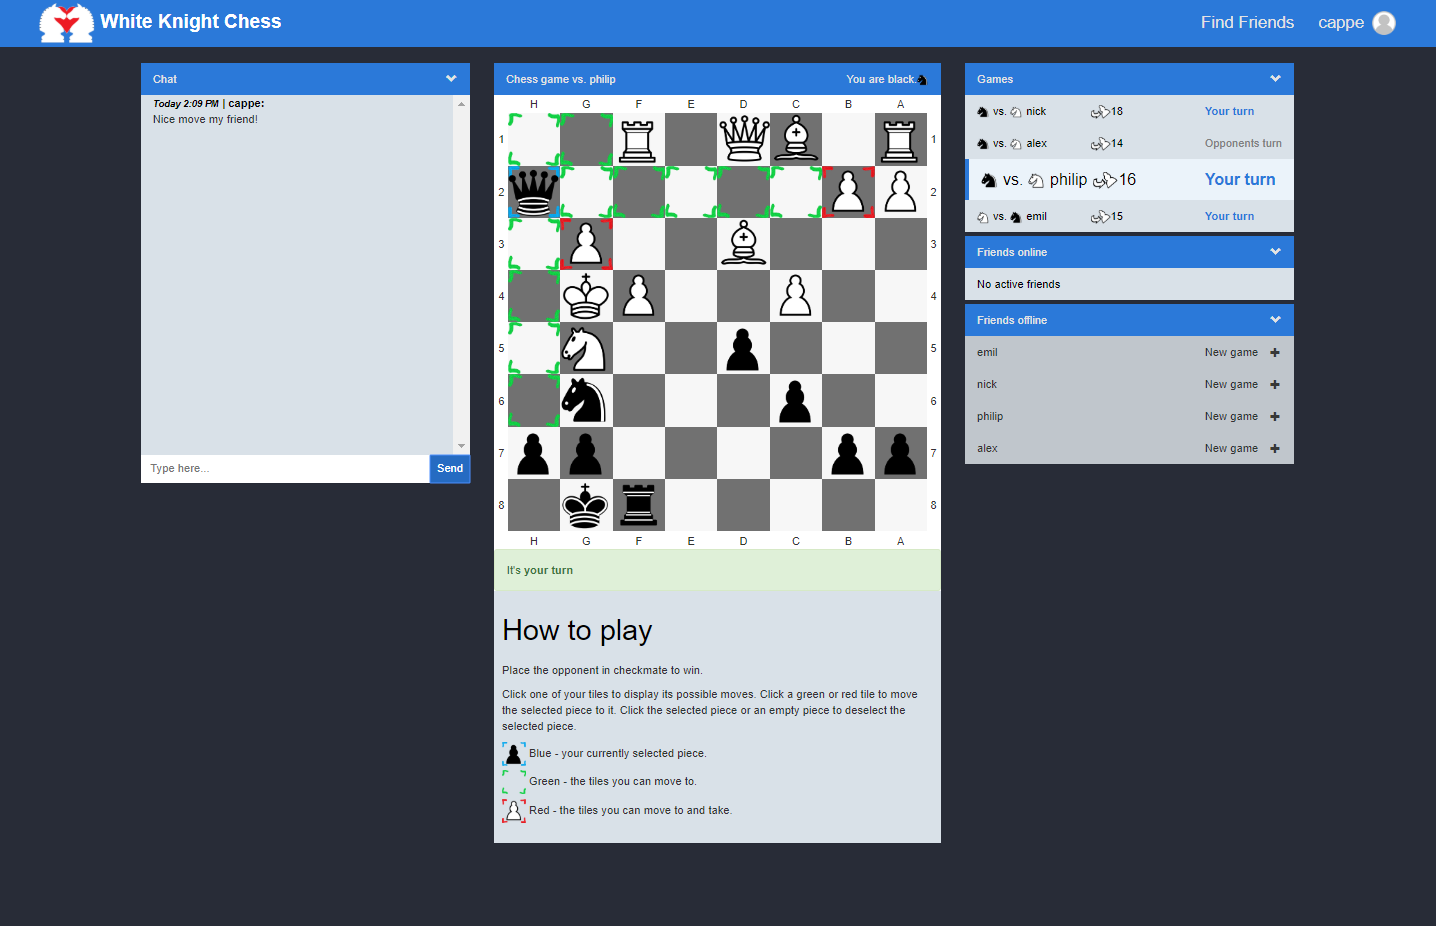
\includegraphics[width=\textwidth]{images/screenshot-of-WKC.png}
  \Description{White Knight Chess game view}
  \caption{The game view as seen by the user “cappe” engaged in a chess match against “philip”. On the top is the navigation-bar. On the left is the chat for the game, and the game itself is shown in the middle. Possible moves for the selected piece (highlighted in blue) are highlighted in green and red. In the sidebar, links to and information about other games “cappe” is engaged in can be seen, as well as his friends.
  }
  \label{fig:game-view}
\end{figure}

\section{Background}
Related websites which inspired this work are chess.com and lichess.org\cite{chess.com, lichess.org}. These sites feature the ability to view completed games and start new games with friends from your friends list. Some of the features these sites contain are: leaderboards, different game modes, highlighting for all possible moves for a selected piece, and the possibility of playing against a computer. (EE, PK, AA)

White Knight Chess (referred to as WKC from now on) is a web application for playing chess against friends or other users. One core feature is a secure account system. Users can manage their account by changing password on the profile page, where there also is an archive for completed games. WKC supports a large player base, because the software is scalable. The landing page shows the lobby, containing all users looking for an opponent. While playing (fig. \ref{fig:game-view}), users are informed when they are checked and if it is their turn. WKC also has a chat for each game and a friend system. From the search page, users can search for and add other users as friends. There is also a sidebar available throughout the site. It shows information about the user’s active games, and shows both online and offline friends. From here new games can be started. The website is mobile and tablet friendly, with layouts for three different screen sizes. Several frameworks and design patterns were used to build WKC. (EE, PK)

Bootstrap is a popular front-end framework for HTML, CSS, and JavaScript for developing responsive, mobile friendly web pages\cite{bootstrap}. Bootstrap takes the mobile-first approach to its design\cite{responsive-web-design}. This means the framework supports smaller devices and less feature-rich browsers that might not understand JavaScript or media queries, but also seamlessly adapts to larger devices and feature-rich browsers. (PK, EE)

The ASP.NET Core MVC framework is based of the MVC design pattern\cite{aspnet-mvc}. MVC stands for Model-View-Controller, which is a separation of concerns between the View, responsible for producing HTML markdown for the clients; the controller, responsible for handling HTTP requests from the client to the server (routing); and the Model, which contains the business logic and data that is used between the View and Controller. MVC allows for hiding the underlying structure of data to the client. It aims to provide a clean separation of concerns. (PK, CA)

ASP.NET Identity is an extensible user account system that plugs into any .NET application\cite{aspnet-identity}. It offers a prebuilt template with secure login and management pages. It comes with a login/register system and a “remember me” functionality. This includes hashing the passwords and saving them to a database, and setting a persistent cookie that expires after two weeks to remember that you were logged in. (PK, CA, NG)

ASP.NET Identity makes use of Microsoft’s ADO.NET Entity Framework (EF Core) by default\cite{adodotnet}. EF Core is an Object-Relational-Mapping database (ORM), meaning it automatically translates C\# classes into database tables and the other way around when querying data. Using an ORM comes with the cost of understanding the actual structure of the database and schema\cite{orm}. However, EF Core supports easy use of C\#’s LINQ library which automatically protects against SQL injection\cite{ef-linq}. LINQ makes it easier to write SQL queries, without a need to convert the received data. (CA, PK)

A Repository is an object or component that acts as an intermediary between the model layer and data layer by centralizing all data access and encapsulating the logic required to access data sources\cite{Repository-pattern}. By encapsulating objects stored in the database together with operations that can be performed on them, the data source is decoupled from the model. This can result in better maintainability and easier testing, as the repository could easily be changed. (AA, PK)

Dependency injection allows for easy module replacement\cite{dependency-injection}. By pre-defining the controllers' behaviour towards the different modules, using interfaces, any class that implements the interface can be injected. This allows for data hiding and testing of different implementations or temporary mock-data. (PK, CA)

Data Transfer Objects (DTOs) are used to transfer data in a single object. They can limit the number of calls to the server\cite{DTOs}. Instead of calling the server for each atomic data, the server can collect the information into one DTO and send it to the client. DTOs are therefore convenient when handling large amounts of data or nested structures. (NG, PK)

The observer pattern consists of one subject object and several observer objects which are notified when something changes in the subject\cite{Design-patterns}. This is commonly used on a higher level of abstraction with a standard library. (PK)


\section{Code structure}
WKC consists of three main components: Data, which handles the database; Game, for the gamelogic; UI, which handles client requests and contains all web pages. 

The Game and Data components are built as standalone projects with their own namespaces. This facilitated separate testing. The UI component is the web server that actually serves the clients and references the other two components. Each component contains the models and entities for the data required for its internal operations. We decided the Game and Data components should not reference any other projects, in order to reduce problems from people working on different code. The UI however, uses data models from Game and Data.

\begin{figure}
  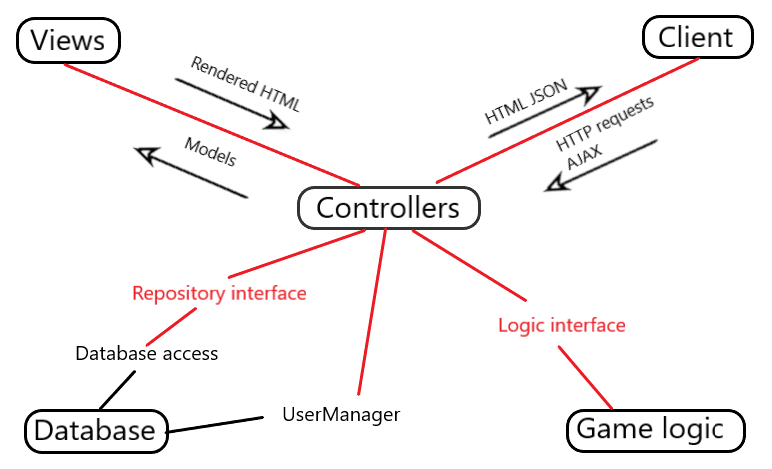
\includegraphics[width=\textwidth]{images/image3.png}
  \Description{Code structure}
  \caption{Illustration of the project layout and interaction between different components. The MVC pattern is present in the Controllers processing requests and passing Models to the Views, which are then sent to the client.
  }
  \label{fig:project-layout}
\end{figure}

We injected both the gamelogic and the database repository as dependencies into the controllers which needed to use them (fig. \ref{fig:project-layout}). UserManager is part of the ASP.NET Identity System and is also injected. It provides methods for working with users, for example, getting the user ID for the client sending a request. (CA, PK)



\section{Method}
  \subsection{Setting up the project}
    We first had a design meeting, discussing how the end result should look and feel. After reviewing related websites we formulated a basic design for the layout of the necessary visual artifacts. We chose to use the ASP.NET MVC framework because we were familiar with it. We planned to first build a functional foundation, and then add new features in iterative steps. Then we split the project into three major components. Game, data, and user interface, as described in the previous section. We agreed to use Git as version control and proceeded to set up a Git repository on GitHub. We then made a weekly schedule so that each group member would partake in at least 16 hours of development sessions weekly. We decided who would be responsible for which part of the project. (PK, NG, CA)

    Nick and Emil were assigned to work on the user interface. Nick has previously redesigned the KronoX app, and Emil has experience with web design from previous education\cite{nick}. Alexander opted for the data component, since he has used EF Core in the laborations of this course. Casper was a good fit for the game component, since he is productive independently. Philip became the project manager, because he has had similar roles previously. We wanted to have a project manager to circumvent the tardiness problem of direct democracy that we experienced in previous projects. It became Philip’s responsibility to review the code that was pushed to the master branch, and to make sure that we followed the project plan and  good practice. (PK, NG)

    Initially, we worked in one branch for each of the three groups and made pull requests to the master branch on GitHub. After the first week, we switched to the GitHub Flow workflow\cite{githubflow}. This allowed us to work on feature branches, which after review can be merged to master with the newly implemented feature. (NG, PK)

    For data storage, we used a Microsoft SQL database coupled with EF Core because of its ease of use and our previous experience with it. EF Core facilitated the code-first approach to generate the database schema. This reduced our workload to set up a database by abstracting the database design. This choice to use EF Core removed the necessity to manually write SQL queries which is both error-prone and vulnerable to SQL injection. We could instead use LINQ to write strongly typed queries. We used the repository pattern in our project to abstract and encapsulate the database and make the data accessible through an interface. It also gives the project better maintainability and helps achieve a higher state of modularity, and less coupling. Using a repository makes it easy to change database provider. For example, Casper could work on a Linux computer with a SQLite database. (AA, PK)


  \subsection{Implementing features}
    We then started implementing the lobby. When a user requests to join the lobby a method is called which changes the user's lobby status to “Registered” in the database. To leave the lobby another method is called that changes the status again. A user will also be automatically removed from the lobby when another user joins their game from the lobby. The lobby view is refreshed with AJAX so that changes in the lobby are visible to the user. (NG, EE, PK)

    The board is first rendered when a specific game session is requested by the client. Razor code, which is C\# code compiled on the server but written inline with HTML markdown, is used to draw the board state of the game session\cite{razor}. Information about the user is also accessed by the Razor code in order to draw the board from each player's point of view. This is done by generating 64 css-grid styled div-tags which display images for the pieces. To make the board responsive, we implemented a naive version of the observer pattern in AJAX\cite{ajax}. Each web-client is an observer, waiting for the state of the board to change. This is more efficient than constantly updating the entire board, regardless if it is changed or not. An \textit{event loop} (implemented as a timed javascript function) makes a request to the \textit{event provider} (a POST request to the back-end)\cite{event-loop}. If changes have been made, another javascript function is called to \textit{dispatch} the event, by updating the affected tiles’ div-tags. In a non-distributed application an event loop might not have a timer, but on a web application it conserves bandwidth. By only refreshing the affected tiles, less client resources are used and the user experiences a responsive interface. (PK)

    We built a chess engine to separate the game logic into its own component that is ignorant of the rest of the application. Therefore it could well be used for a non-web related project. It needs to know the state of the board, whose turn it is, and which tile is selected or what move the player wants to do. This is provided by DTO parameters. The game component can:
    \begin{itemize}
      \item decide if a move is valid.
      \item provide a list of valid moves for a piece.
      \item perform a move and return the new state of the board.
      \item decide if a player is checked or in checkmate.
    \end{itemize}
    
    We implemented functions to get the basic valid moves for each type of chess piece from its current position. Using this we could get all the opponent’s valid moves. If the king is in one of those positions the player is checked. To see if the player is in checkmate every possible move for the player is also evaluated to decide if the player would still be checked if making that move. If no move can stop the king from being checked the player is in checkmate and the game is over. (CA, PK)
    
    After our second meeting with Rong, we were required to implement a chat-system for grade 5. First we researched a chat system with a hub connection that was part of the ASP.NET SignalR library\cite{signalr}. However, we would not have time to learn it and adapt it to the project. We instead implemented a new chat system with AJAX, which we knew how to do. We stored the chat messages in a table with a foreign key to a particular gamesession, which meant that a chat message and a gamesession have a many-to-one relationship. The message and game ID is sent with a POST request to a controller, which adds a timestamp and a username to the object and saves it to the database. Our javascript periodically polls the server if the chat has been updated with a POST request. If it has been updated, the partial view of the chat is reloaded asynchronously to fulfill our vision of fluency and responsiveness. Without AJAX the user would have to refresh the page every time they wanted to see if the chat is updated. That is why this feature was deemed more important than features we didn't implement, mentioned in the discussion. (NG, CA, PK)

    We realized the users might expect to access their games after they are finished. Since they will no longer appear in the sidebar of active games, we implemented an archive. The archive uses a partial view of the game board to display the state the game was in when it ended. This reuses much of the code used to draw the board. The repository also provides a list of finished games for the signed in user of which one game can be shown at a time. (NG, PK)



  \subsection{User study}
    To evaluate our website a user study was performed on two anonymous participants. All participants were informed beforehand of their rights to withdraw consent, and that the results would be used for a project report. The participants were asked to perform tasks that test the core functionality and features of our website. Then the participants were asked about their experience. These questions allowed us to receive feedback on both the functionality and the design of our website, and highlight areas in need of improvement. 

    They were tasked to:
    \begin{enumerate}
      \item Create a new account.
      \item Start a new game from the lobby page.
      \item Make the first move in the game.
      \item Add a user as a friend.
      \item Start a new game with that user.
      \item Log out.
    \end{enumerate}

    They were then asked these questions:
    \begin{enumerate}
      \item Did you have any problems performing the tasks? Was it unclear how to execute any of the tasks?
      \item Do you have any general feedback or opinions of the website?
      \item If there is one thing you could change about the website, what would it be?
    \end{enumerate}

    No user found the tasks difficult to complete. They found the website was aesthetically pleasing. One user asked for a help button to display what certain things do and how they work. One user experienced that it was odd to see an empty chat when entering a new game. (EE, NG, PK)



\section{Discussion}
  During the user study no participants had problems navigating the website. The information provided on each page seemed to be sufficient as they quickly understood the core functionality of each page. One user said that they wanted a help-button that provides useful information or tips when clicked. This tells us that the user experience might be improved by giving first time users access to more information if they want it. The chat window on the game page starts out as an empty window. An improvement might be to make the window smaller at first, only expanding with new messages. (EE, PK)

  WKC can be developed further by improving existing features, as well as adding new features. Possible new features include customizable appearance, better notifications, move history, a leaderboard, extended user statuses, persistent friend-to-friend chats, and more efficient game logic. (EE, PK)

  During our presentation we received feedback from Afshin that users might want more noticable indications of when a message is received or a game status is updated by way of a notification. The sidebar of the website currently shows the status of every game that a user is playing. When the opponent makes a move the sidebar dynamically updates to show that it is your turn. An improved system could show a notification as well, and prompt users to accept or decline friend- and game requests. This would improve the user experience by making relevant information more accessible, in a manner that most users will be familiar with from their experience with smartphone operating systems. (EE, NG, PK)

  Another extension of the archive would be a history of every move in the game. This would also show the state of the game for each move. The move history would be displayed next to the game board so a user can see the history of the game, both in the archive view and while playing an ongoing game. This implementation would help players master chess by going back to analyze their moves. (EE, NG, PK)

  Rong suggested during a meeting that an improvement of the chat, in general the dynamic parts, could be made by using the publish-subscribe pattern. This can be achieved with ASP.NET SignalR library and allow us to remove the AJAX that runs at timed intervals, and replace it with publishing when a change is made on the database\cite{signalr}. The client would not have to rely on an interval to wait for the next fetch attempt, and there would not be constant requests to the server. (PK, NG)

  Other than “online” and “offline", there could be another status for when a user has been inactive for some time, but are still logged in. This status could be displayed as “away”, and would indicate if a friend is available. (EE, PK)

  The current game logic uses a naive and inefficient method for finding checkmate. There are duplicate checks done. These unnecessary calculations use processing power that could be used for other computations. This could become a severe problem if there are many users. Also, if a scalable cloud service hosts the server, inefficient code leads to higher operating costs. Instead of attempting every move for each piece, we can use a process of elimination by starting with a collection of every tile the enemies that are checking the king are standing on and can move to and remove every tile that doesn't solve the problem. Also, instead of creating a copy of the original board every time, it would be better to use one board to do a move and then backtrack it after each attempted move. (CA, PK)

  \bibliography{sources}

\end{document}